\chapter{Descrição do Estudo Proposto}\label{cap:estudo-proposto}
\graphicspath{{chapter-06/img-cap06/}}

No presente trabalho serão ilustrados e analisados os resultados obtidos pelas análises numéricas computacionais para um escoamento compressível, axissimétrico e em regime permanente baseado na abordagem RANS para descrever a turbulência, em especial os modelos Spalart-Allmaras e SST $\kappa$-$\omega$. Dentre os trabalhos já citados, as referências \cite{Dali2018a,Sahu1985,Mahmoud2009,torangatti2basawaraj,belaidouni2016,nicolas-perez_accuracy_2017,Lucena2020,Reddy2021} serviram como norteadoras para o emprego dessas simulações. 

Ademais, a implementação do MPMTM faz uso dos recursos disponíveis pelas simulações CFD a fim de comparar o funcionamento do projetil em duas situações: o voo inerte, que seria o voo sem uso do \textit{Base Bleed}; voo ativo, com o uso do \textit{Base Bleed}. Desta forma, aplica-se o que já foi desenvolvido e consolidado em trabalhos anteriores \cite{Rosendo2020,Gauchoux1991,balon2006analysis,Abou-Elela2013,Skande2014,Lim2016}.

\section{Parâmetros de Interesse}

Nesta seção espera-se definir quais variáveis de saída são relevantes para o projeto. Por razões técnicas, a tecnologia \textit{Base Bleed} procura resolver o problema do arrasto induzido na base do projetil, logo são calculados os valores necessários para a compreensão desta força aerodinâmica. 

\subsection{Coeficiente de Arrasto}

Esse coeficiente ($C_D$) é um número adimensional que pode ser obtido de acordo com a equação \ref{eq:cd}:

\begin{equation} \label{eq:cd}
    C_{D} = \frac{F_{D}}{\frac{1}{2}\rho V^2 A}
\end{equation}
%
os termos $F_{D}$, $\frac{1}{2}\rho V^2$ e $A$ representam, respectivamente, a força de arrasto aerodinâmico, a pressão dinâmica exercida pelo fluido e a área de referência da munição. Neste trabalho em específico, não são considerados os efeitos causados pelo ângulo de ataque.

\subsection{Coeficiente de Pressão}

A pressão é uma das propriedades de maior interesse do fluido, portanto calcula-se um adimensional que permite entender como as forças de sustentação e arrasto se comportam no escoamento. O coeficiente de pressão ($C_{P}$) é um número adimensional que descreve as pressões relativas no escoamento independente do tamanho do corpo. Ele pode ser calculado a partir da expressão \eqref{eq:cp-equation}: 

\begin{equation}\label{eq:cp-equation}
    C_P = \frac{p - p_{\infty}}{\frac{1}{2}\rho V^2}
\end{equation}
%
onde $p_{\infty}$ é a pressão do meio livre. Quando os contornos de pressão indicam regiões com $C_{P} > 1$, o escoamento é compressível.

\subsection{Parâmetro de Injeção}

Para aplicar o conceito do parâmetro, $Inj$, é necessário olhar para a equação \ref{eq:parametro-injecao}:

\begin{equation}\label{eq:parametro-injecao}
    Inj = \frac{\Dot{m}_{BB}}{\rho VA_{b}}
\end{equation}
%
onde $A_{b}$ significa a área da base do projetil. 

Ao observar a equação \ref{eq:parametro-injecao}, o maior desafio é obter valores razoáveis para a injeção de gases na base do projetil, pois o $Inj$ tem influência na equação \ref{eq:baseMPM}. Para isto, deve-se ter em mãos os valores de vazão mássica do propelente injetado pelo sistema BB, $\Dot{m}_{BB}$. Como o fluido de trabalho é considerado ideal, portanto a vazão mássica pode ser calculada através da equação \ref{eq:vazao-massica-BB} \cite{Gil2020}:

\begin{equation}\label{eq:vazao-massica-BB}
    \Dot{m}_{BB} = \rho_{t}A_{t}V_{t} = \frac{p_{c}A_{t}}{\sqrt{\gamma RT_{c}}}\sqrt{\frac{2\gamma^{2}}{\gamma - 1}\left(\frac{p_{t}}{p_{c}}\right)^{2/\gamma}\left[1-\left(\frac{p_{t}}{p_{c}}\right)^{(\gamma-1)/\gamma}\right]}
\end{equation}
%
Sejam $p_{c}$ e $p_{t}$ as pressões na câmara geradora de gás e na saída do sistema, respectivamente. Os termos $\rho_{t}$, $V_{t}$ e $A_{t}$ se referem a densidade, a velocidade e a área na saída do \textit{Base Bleed}. 

Como requisitos das simulações de dinâmica dos fluidos computacional, a temperatura e velocidade de saída dos gases (em função do número de Mach) são computadas com base na pressão da câmara, que é obtida a partir da equação \ref{eq:vazao-massica-BB}. Como o gás é isentrópico, as equações para essas propriedades são as seguintes:

\begin{align}
    \label{eq:temperatura-BB}
    T_{t} = T_{c}\left(\frac{p_t}{p_c}\right)^{(\gamma - 1)/\gamma} \\
    \label{eq:velocidade-mach-BB}
    M_{t} = \sqrt{\frac{2}{\gamma - 1}\left[\left(\frac{p_c}{p_t}\right)^{(\gamma - 1)/\gamma}-1\right]}
\end{align}

\section{Geração de malha}\label{sec:geracao-malha}

Para conseguir formular a abordagem numérica exigida pelo método de volumes finitos, a ser empregado no presente trabalho, foi necessário construir um domínio computacional através de uma malha. Com a evolução do projeto, foi construída um domínio axissimétrico em formato de "C", assim como visto em trabalhos anteriores \cite{Mahmoud2009,nicolas-perez_accuracy_2017}. Uma vantagem desse tipo de malha é permitir simplificações nas fronteiras para imposição das condições de contorno, além de reduzir o custo computacional para obtenção de resultados.

\begin{figure}[!ht]
	\centering
	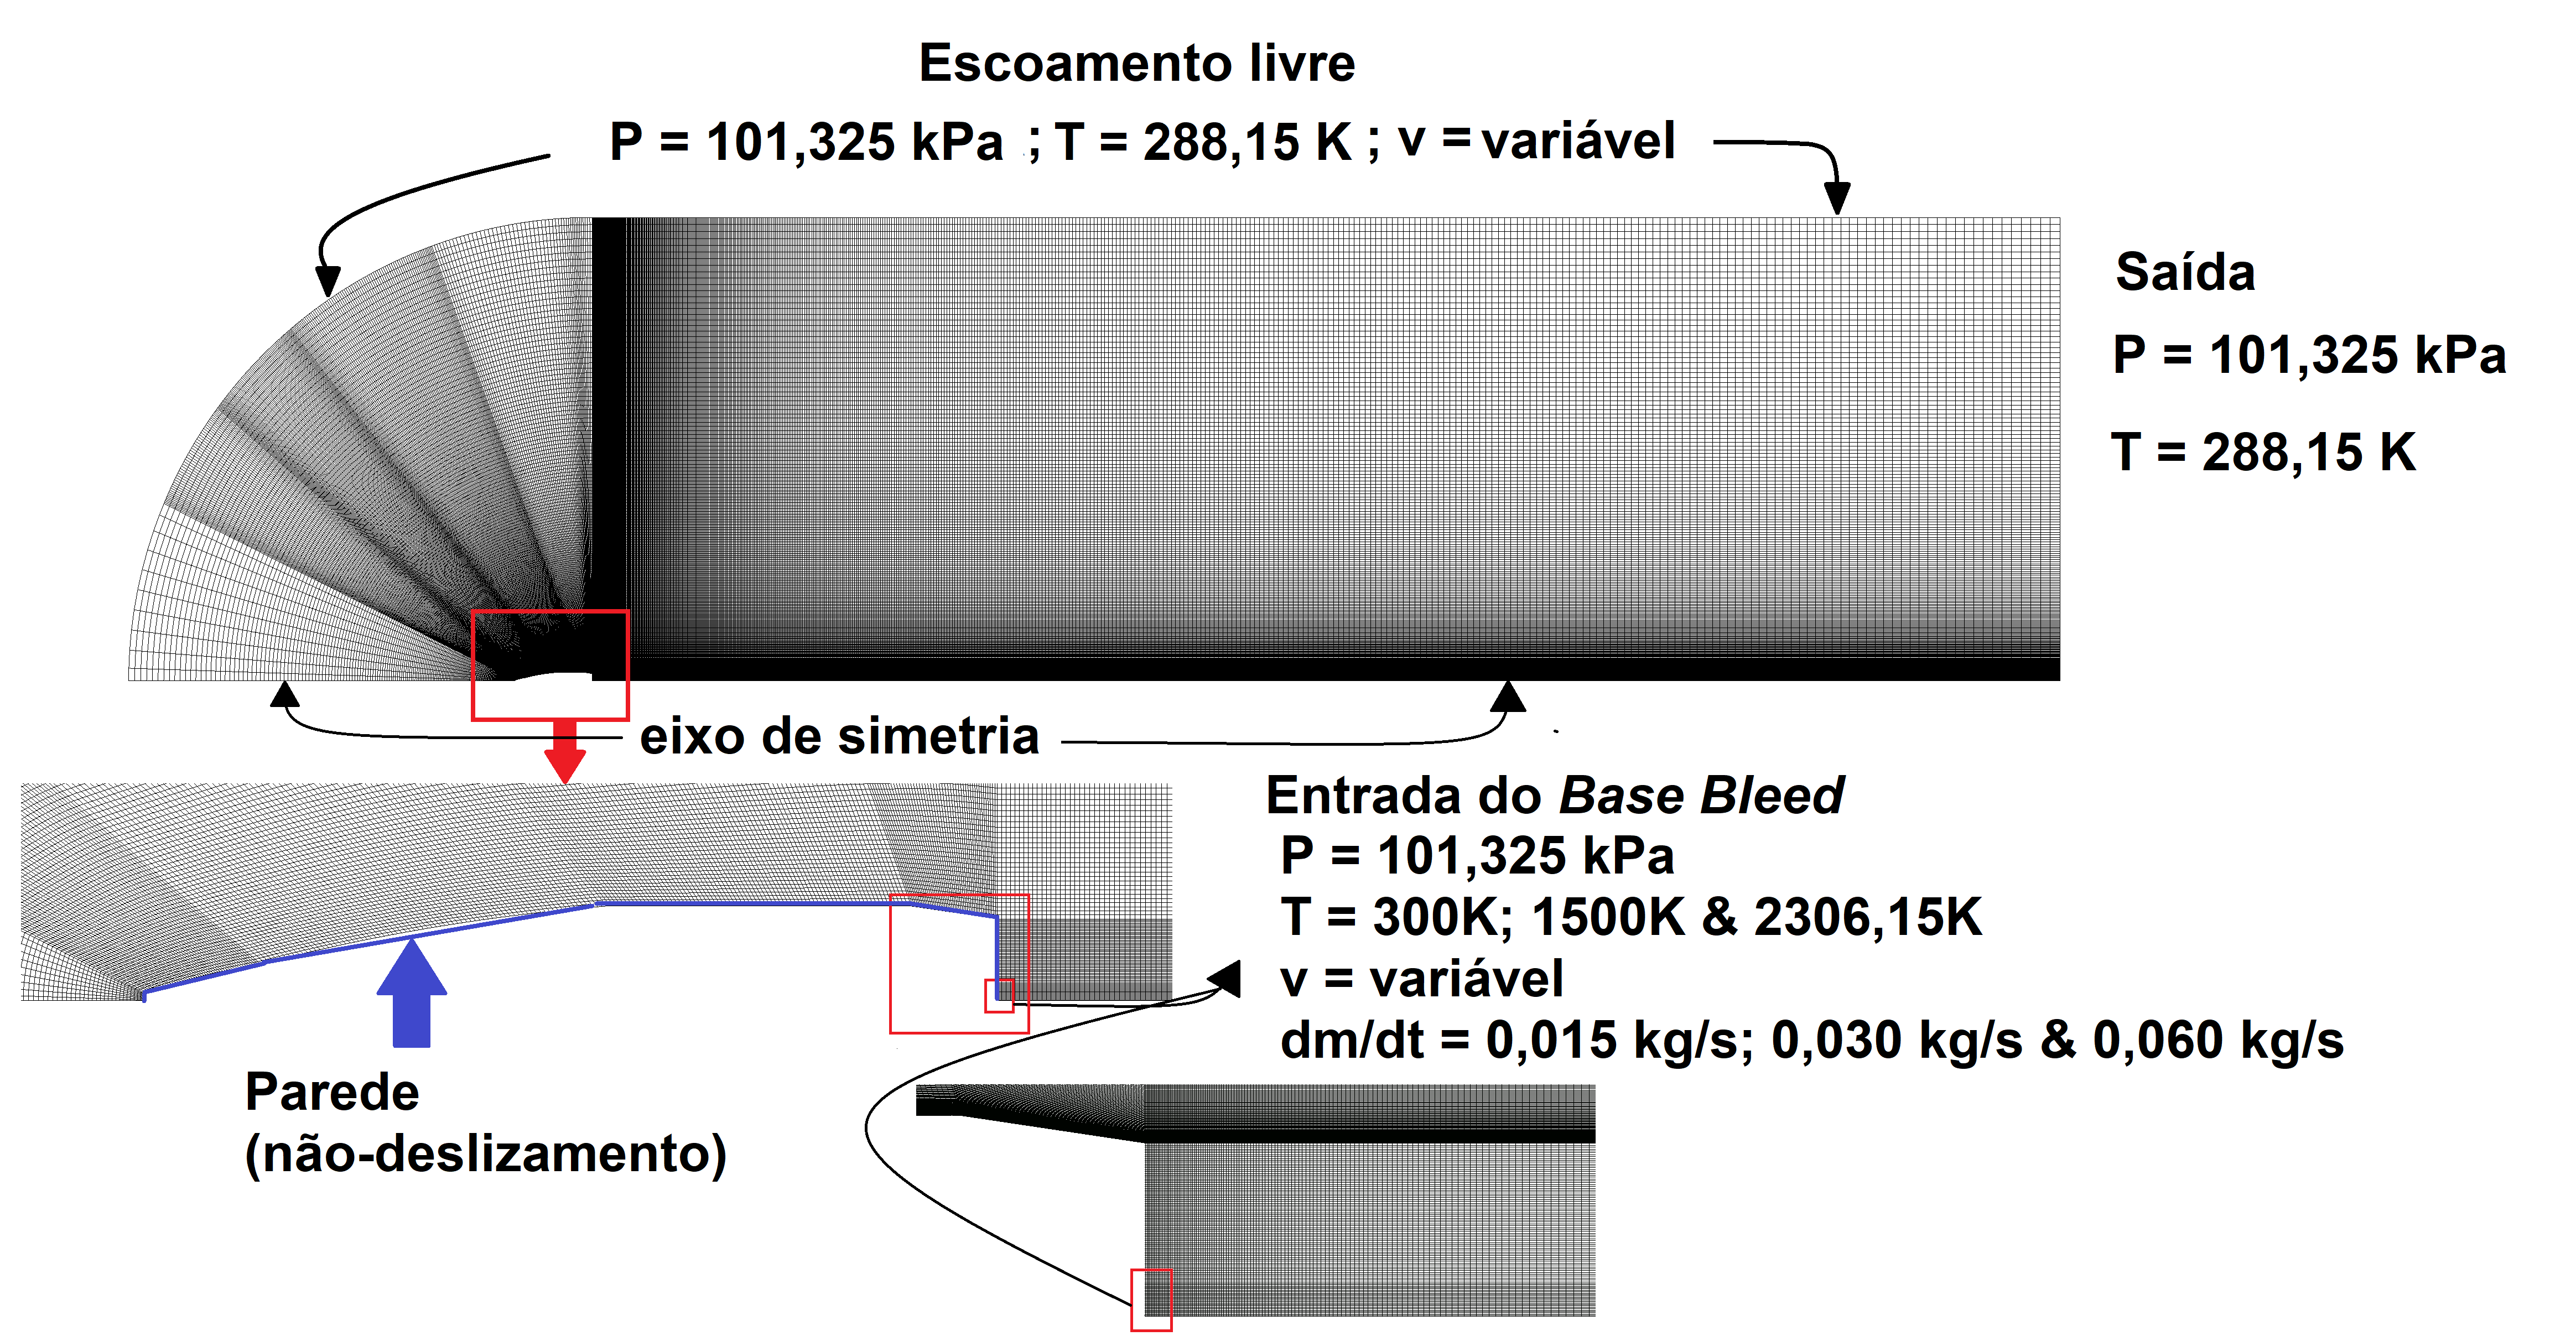
\includegraphics[width=1.0\textwidth]{foto01-malha.png}
	\caption{Domínio computacional}
	\label{fig12:autor-malha}
\end{figure}

E com o domínio preparado, foram feitas 2 malhas (vide Tabela \ref{tab:tabela-malhas-inicial}), objetivando comparar valores com referências já citadas \cite{Mahmoud2009} para obter convergência dos resultados. Na direção vertical, a maior distância ao projetil é da ordem de 20 vezes o próprio calibre, enquanto que na direção horizontal à montante a maior distância ao projetil ficou na ordem de 5 vezes o comprimento longitudinal e à jusante na ordem de 15 vezes o valor do comprimento de referência da munição. Em ambos os casos, o diâmetro de saída do bocal do sistema \textit{Base Bleed} é de \qty{1}{\polegada} (\qty{25,4}{\millimetre}).

\begin{table}[ht]
\centering
\caption[Malhas desenvolvidas para o domínio computacional (sem \textit{Base Bleed})]{Malhas desenvolvidas para o domínio computacional (sem \textit{Base Bleed})}
\vspace{0.5cm}
\begin{tabular}{c|c}
\multicolumn{2}{c}{1\textsuperscript{o} Teste de Convergência} \\
\hline 
Número da Malha & Quantidade de elementos \\ 
\hline
1 & \num{186500} \\
2 & \num{380000}
\end{tabular}
\label{tab:tabela-malhas-inicial}
\fonte{Autor.}
\end{table}

A seguir a segunda fase de testes de convergência foi realizada, assumindo que o diâmetro de saída do bocal do sistema BB seja igual a \qty{50,8}{\millimetre} e a temperatura de saída com valor de \qty{2306,15}{\kelvin}. Nesta etapa, foram testadas 4 malhas, de acordo com a Tabela \ref{tab:tabela-malhas-secundaria}, com a finalidade era ratificar a suficiência da malha com \num{380000} elementos para obtenção dos resultados finais.

\begin{table}[ht]
\centering
\caption[Malhas desenvolvidas para o domínio computacional (com \textit{Base Bleed})]{Malhas desenvolvidas para o domínio computacional (com \textit{Base Bleed})}
\vspace{0.5cm}
\begin{tabular}{c|c}
\multicolumn{2}{c}{2\textsuperscript{o} Teste de Convergência} \\
\hline 
Número da Malha & Quantidade de elementos \\ 
\hline
1 & \num{380000} \\
2 & \num{453600} \\
3 & \num{514800} \\
4 & \num{566550}
\end{tabular}
\label{tab:tabela-malhas-secundaria}
\fonte{Autor.}
\end{table}

Após a ratificação dos valores encontrados para o coeficiente de arrasto, atestou-se a influência do efeito \textit{Base Bleed} pela temperatura de injeção dos gases. É importante salientar que a maior temperatura foi extraída de outro trabalho desenvolvido pelo autor desta dissertação em que se fez presente como co-autor \cite{Gil2020}.

\begin{table}[ht]
\centering
\caption[Efeito \textit{Base Bleed} em função da temperatura]{Efeito \textit{Base Bleed} em função da temperatura}
\vspace{0.5cm}
\begin{tabular}{c|c}
Diâmetro do Base Bleed & Temperatura\\ 
\hline
\multirow{3}*{\qty{25,4}{\millimetre}} & \qty{300}{\kelvin}\\
& \qty{1500}{\kelvin}\\
& \qty{2306,15}{\kelvin}
\end{tabular}
\label{tab:tabela-bb-temperatura}
\fonte{Autor.}
\end{table}

Após esse passo, foram comparados dois diâmetros possíveis para saída da câmara geradora de gás (sistema BB) com a mesma temperatura ($T_{BB} = \qty{2306,15}{\kelvin}$), conforme a Tabela \ref{tab:tabela-vazoes-por-diametro}.

\begin{table}[ht]
\centering
\caption[Diâmetros testados para analisar o efeito \textit{Base Bleed}]{Diâmetros testados para analisar o efeito \textit{Base Bleed}}
\vspace{0.5cm}
\begin{tabular}{c|c|c}
Diâmetro do \textit{Base Bleed} (mm) & Vazão nº1 & Vazão nº 2\\ 
\hline
\qty{25,4}{\millimetre} & \qty{0,015}{\kilogram\per\second} & \qty{0,030}{\kilogram\per\second}\\
\qty{50,8}{\millimetre} & \qty{0,030}{\kilogram\per\second} & \qty{0,060}{\kilogram\per\second}\\
\end{tabular}
\label{tab:tabela-vazoes-por-diametro}
\fonte{Autor.}
\end{table}

\section{Condições de Contorno}\label{sec:condicao-contorno}

No local descrito como "Escoamento livre"{} (\textit{far-field}), o conceito por trás dessa condição é definir o meio livre do escoamento e, como requisito do software comercial utilizado, se fez necessário tratar o fluido (ar) como gás ideal. A pressão $p = \qty{101,325}{\kilo\pascal}$ e a temperatura $T = \qty{288,15}{\kelvin}$ são prescritas de acordo com as condições ambientais para um disparo a nível do mar. A velocidade é prescrita conforme os valores de entrada do escoamento, variando o número de Mach de \numrange{0,4}{3}. 

A região denominada "Saída do \textit{Base Bleed}"{} (\textit{Base Bleed inlet}) mostrada na figura anterior representa a entrada de fluxo de gases injetados na base do projetil, onde a velocidade de entrada possui valor apenas na direção axial. A vazão mássica e a temperatura do BB foram prescritas para descobrir a velocidade do escoamento nesta região. A pressão na saída dos gases BB é definida como sendo igual a pressão no "Escoamento livre"{} $\left(\nabla p = 0\right)$.

No local descrito como "Saída"{} (\textit{outlet}) são prescritas apenas a pressão e a temperatura do contorno, que são iguais aos valores determinados no "Escoamento livre"{} $\left(\nabla p = 0, \nabla T = 0\right)$.

A região da parede, que descreve o contorno do formato do projetil, possui a condição de não-deslizamento, portanto $V_{parede} = 0$ para desconsiderar o efeito dissipativo causado pela rugosidade da superfície. A parede é considerada como adiabática, logo o fluxo de temperatura nesta região é nulo $\left(\nabla T = 0\right)$.

Há a referência para o eixo de simetria, a fim de se garantir que os cálculos sejam feitos de acordo com o estudo proposto. Em todas as regiões definidas o valor da intensidade de turbulência determinado é de 0\% e o comprimento da escala turbulenta igual a \qty{0,7}{\metre}, aproximadamente o valor do comprimento do projetil.

\section{Método de Resolução das Simulações CFD}\label{sec:metodo-resolucao-cfd}

Em todos os casos simulados no presente trabalho foi utilizado o método numérico denominado método dos volumes finitos \cite{McDonald1971,MacComarck&Paulay1972} para discretizar as equações de governo. O esquema de interpolação para os termos advectivos e difusivos foi o \textit{upwind} de 2\textsuperscript{a} ordem. 

Para lidar com a compressibilidade existente no regime de voo desta munição estudada, o esquema \textit{density-based} totalmente implícito foi aplicado \cite{Weiss1995PreconditioningAT,Weiss1997IMPLICITSO,Weiss1999ImplicitSO}. Em todos os casos simulados o regime estacionário foi considerado, portanto as propriedades calculadas não variam em função do tempo. 

Para o cálculo dos gradientes foi utilizado o método dos Mínimos Quadrados e o esquema de avaliação do fluxo optou pelo ROE-FDS, pois demonstra bons resultados para problemas com escoamentos compressíveis \cite{nicolas-perez_accuracy_2017}. Para a resolução do sistema de equações lineares foi utilizada a técnica \textit{multigrid} \cite{Hutchinson1986}.

O problema foi considerado convergido quando todos os resíduos forem menores que $\num{1e-6}$. Um software comercial foi usado para a construção da geometria, construção das malhas, além de suporte aos métodos numéricos e equações de governo e no pós-processamento dos casos construídos \cite{fluent2021ansys}.

\section{Implementação do Modelo de Trajetória}\label{subsec:implementacao-trajetoria}

No trabalho de \citeauthor{Rosendo2020} cita-se a necessidade de dividir os dados de entrada relevantes de projeto em 4 grandes seções: aerodinâmicos, ambientais, balísticos e geométricos. A Figura \ref{fig:fluxograma-mpmtm} apresenta o fluxograma com as condições necessárias, que são apresentadas da \autoref{subsec:condicoes-geometricas} a \autoref{subsec:condicoes-aerodinamicas}, bem como a aplicação do integrador numérico Runge-Kutta de 4\textsuperscript{a} ordem, anteriormente explicado na \autoref{sec:numint}. Destaca-se três pontos importantes: as funções para o parâmetro de injeção e a guinada de repouso, pois são parâmetros essenciais ao projeto e permitem calcular o desempenho da munição com e sem \textit{Base Bleed}, além da definição da altura que o projetil atinge o solo, pois serve como limitador do processo iterativo. 

\begin{figure}[!ht]
	\centering
	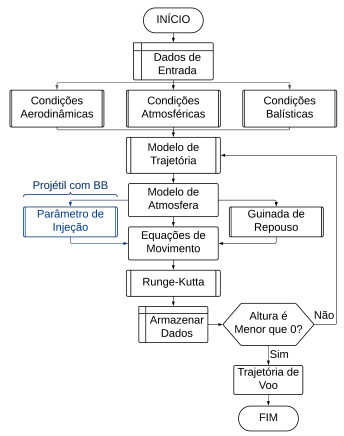
\includegraphics[width=0.6\textwidth]{foto03-fluxograma-mpmtm.png}
	\caption{Domínio computacional}
	\label{fig:fluxograma-mpmtm}
\end{figure}

\subsection{Condições Geométricas}\label{subsec:condicoes-geometricas}

O projetil de calibre \qty{155}{\millimetre} possui um formato axissimétrico, portanto ele permite aplicar o modelo MPMTM. Isto é, o corpo rígido é tratado como um ponto material. Contudo, o Quadro \ref{quad:geo_inputs} apresenta quais informações são exigidas para implementação do código que calcula a trajetória, conforme previsto pela STANAG 4355.

\begin{quadro}[htb]
\caption{\label{quad:geo_inputs}Dados Geométricos}
\begin{tabular}{|c|c|}
    \hline
    \textbf{Descrição} & \textbf{Valores} \\ 
    \hline
    Diâmetro de referência & \qty{0,15470}{\metre} \\ 
    \hline
    Diâmetro do boat-tail & \qty{0,13373}{\metre} \\ 
    \hline
    Massa (sem propelente) & \qty{42,9850}{\kilogram} \\ 
    \hline
    Massa do propelente & \qty{0,5600}{\kilogram} \\ 
    \hline
    Momento de inércia axial no início & \qty{0,14245}{\kilogram\per\square\metre} \\ 
    \hline
    Momento de inércia axial após a queima & \qty{0,13730}{\kilogram\per\square\metre} \\
    \hline
    Centro de gravidade no início (a partir da ponta da ogiva) & \qty{0,45835}{\metre} \\
    \hline
    Centro de gravidade após a queima (a partir da ponta da ogiva) & \qty{0,44645}{\metre} \\
    \hline
\end{tabular}
\fonte{Autor.}
\end{quadro}

\subsection{Condições Balísticas}\label{subsec:condicoes-balisticas}

\begin{figure}[!ht]
	\centering
	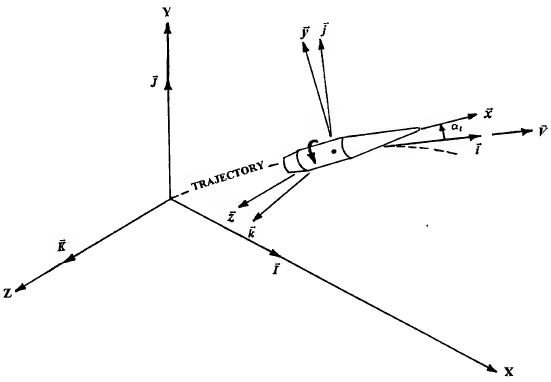
\includegraphics[width=0.5\textwidth]{foto02-mccoy2012.png}   
	\caption[Sistema de referência para o cálculo de trajetória]{Sistema de referência para o cálculo de trajetória \cite{McCoy2012}}
	\label{fig:traj-ref-mccoy2012}
\end{figure}

Neste sistema o canhão é centrado no eixo de referência da Terra em $O_{\text{XYZ}}$, conforme Figura \ref{fig:traj-ref-mccoy2012} e programado para lançar com ângulos de elevação (QE) de \qtylist{40;45}{\degree} (\qtylist{711,1;800,0}{\milliradian}) a partir da horizontal, partindo com a mesma velocidade (Mach aproximadamente \num{2,58}, a nível do mar). Como citado na \autoref{quad:muzzle_inputs}, os fatores de arrasto e Magnus são constantes expressadas na STANAG 4355. A latitude do Rio de Janeiro foi considerada para vias de estudo.

\begin{quadro}[htb]
\caption{\label{quad:muzzle_inputs}Dados Balísticos}
\begin{tabular}{|c|c|}
\hline
\textbf{Descrição} & \textbf{Valores}\\
\hline
Velocidade de disparo & \qty{878}{\metre\per\second} \\
\hline
Ângulo de elevação & \qtylist{711,1;800,0}{\milliradian} \\
\hline
Latitude & \qty[parse-numbers=false]{-23 \pi/180}{\radian} \\
\hline
Azimute & \qty{0}{\radian} \\
\hline
Taxa de torção no disparo & \qty{25}{\calibers\per\revolution} \\
\hline
Fator de arrasto & 1,2 \\
\hline
Fator de Magnus & 1,2 \\
\hline
\end{tabular}
\fonte{Autor.}
\end{quadro}

\subsection{Condições Atmosféricas}\label{subsec:condicoes-ambientais}

Respeitando o modelo da ICAO \cite{international1993manual}, existem algumas variáveis de interesse no início do lançamento. Elas estão representadas no \autoref{quad:ICAOinputs}. A velocidade do vento foi desconsiderada porque o simulador necessitava criar confiabilidade antes de aumentar as incertezas, assim como os fatores de umidade foram desprezados pela mesma razão.

\begin{quadro}[htb]
\caption{\label{quad:ICAOinputs}Dados Atmosféricos}
\begin{tabular}{|c|c|}
\hline
\textbf{Descrição} & \textbf{Valores} \\
\hline
Temperatura ao nível do mar & \qty{288,15}{\kelvin} \\
\hline
Gradiente de Temperatura & \qty[exponent-mode=scientific]{6,5e-3}{\kelvin\per\metre} \\
\hline
Pressão do ar ao nível do mar & \qty[exponent-mode=scientific]{1,01325e5}{\pascal} \\
\hline
Densidade do ar ao nível do mar & \qty{1,225}{\kilogram\per\metre\cubed} \\
\hline
Razão de expansão adiabática do ar & 1,4 \\
\hline
Aceleração da gravidade ao nível do mar & \qty{9,80665}{\metre\per\second\squared} \\
\hline
Raio da Terra & \qty[exponent-mode=scientific]{6,371e6}{\metre} \\
\hline
Velocidade angular da Terra & \qty[exponent-mode=scientific]{7,292e-5}{\radian\per\second} \\
\hline
\end{tabular}
\fonte{\citeonline{international1993manual}}
\end{quadro}

\subsection{Condições Aerodinâmicas}\label{subsec:condicoes-aerodinamicas}

Com o suporte do PRODAS®, os coeficientes aerodinâmicos foram calculados usando formulações semi-empíricas a partir das propriedades geométricas e de massa do projétil sem alcance estendido. Essas variáveis adimensionais são funções do número de Mach e da guinada de repouso.

A norma compara os coeficientes aerodinâmicos da STANAG 4355 com o que a NACA (Comitê Nacional para Aconselhamento da Aeronáutica) oferece \cite{stanag4355}. Os coeficientes obtidos no PRODAS® são calculados em função dos eixos da munição, enquanto que os valores adimensionais de interesse são em respeito ao vetor de velocidade do centro de massa. Logo, são feitas algumas transformações rotacionais para se chegar nos coeficientes desejados:

\begin{equation}
\begin{aligned}
    C_{D_{0}} &= C_{X_{0}} \\
    C_{D_{\alpha^2}} &= C_{X_{\alpha^2}} + C_{Z_{\alpha}} - \frac{1}{2}C_{X_{0}}\\
    C_{L_{\alpha}} &= C_{Z_{\alpha}} - C_{X_{0}} \\
    C_{mag-f} &= \frac{1}{2}C_{y_{pa}} \\
    C_{spin} &= \frac{1}{2}C_{l_{p}}
\end{aligned}
\end{equation}
%
os valores dos coeficientes que foram aplicados ao modelo de trajetória podem ser vistos do \autoref{apend:apendice-sembb} ao \autoref{apend:apendice-combb-2pol-006}.